\documentclass{article}
\usepackage[utf8]{inputenc}
\usepackage[T1]{fontenc}
\usepackage[brazil]{babel}
\usepackage{geometry}
\usepackage{graphicx}
\usepackage{float}
\usepackage{array}
\usepackage{booktabs}
\usepackage{amsmath}
\usepackage{hyperref}
\usepackage{xcolor}
\usepackage{makecell}
\usepackage{subcaption} % no preâmbulo

\title{Relatório Experimental - Sinais Analógicos, ADC, PWM e DAC }
\author{Ana Beatriz Barbosa Yoshida - RA: 245609 \\ Julio Nunes Avelar - RA: 241163}
\date{10 de Setembro de 2025}

\begin{document}

\maketitle

\section{Objetivos}

\begin{itemize}
    \item Compreender como sinais analógicos são lidos via ADC.
    \item Controlar parâmetros de PWM com o joystick (entrada analógica → processamento digital → saída PWM).
    \item Utilizar filtro RC externo para transformar PWM em sinal analógico.
    \item Verificar a tensão filtrada no ADC e compará-la com o valor esperado pelo duty cycle.
\end{itemize}

\section{Lista de Materiais}

\subsection{Equipamentos}

\begin{enumerate}
    \item BitDogLab
    \item Protoboard Pequena
    \item Multímetro digital
    \item Osciloscópio Digital
\end{enumerate}

\subsection{Componentes}

\begin{enumerate}
    \item Resistor 10k
    \item Capacitor 100nf
    \item Resistor 1k
    \item Jumpers macho macho e macho femeá
\end{enumerate}

\subsection{Opcionais}

\begin{enumerate}
    \item Resistores extras
    \item Capacitores extras
\end{enumerate}

\section{Etapas}

\subsection{Leitura do Joystick}

\begin{itemize}
    \item Usar \texttt{GPIO26} (eixo Y) e \texttt{GPIO27} (eixo X) como entradas ADC.
    \item Conceitos trabalhados:
    \begin{itemize}
        \item Conversão analógico-digital.
        \item Resolução (12 bits = 4096 níveis).
        \item Quantização e relação valor digital $\leftrightarrow$ tensão real.
    \end{itemize}
\end{itemize}

\noindent
\textbf{Exercício}: mover o joystick e observar como o valor ADC varia proporcionalmente.

\begin{itemize}
    \item Mostrar no OLED os valores lidos (0–4095 → 0 a 3,3 V).
    \item Fotografe e comente.
\end{itemize}

\noindent
\textbf{Resposta:} As figuras \ref{fig:foto1} e \ref{fig:foto2} mostram a leitura no OLED em dois casos distintos: no primeiro, com um duty próximo a 0\%, onde o nível de tensão esperado é próximo de 0 V, e no segundo, com um duty próximo a 100\%, onde o valor esperado é próximo de 3.3 V. É perceptível que a leitura não é exata, apresentando uma pequena margem de erro nos valores obtidos.

\begin{figure}[H]
    \centering
    \begin{minipage}{0.45\linewidth}
        \centering
        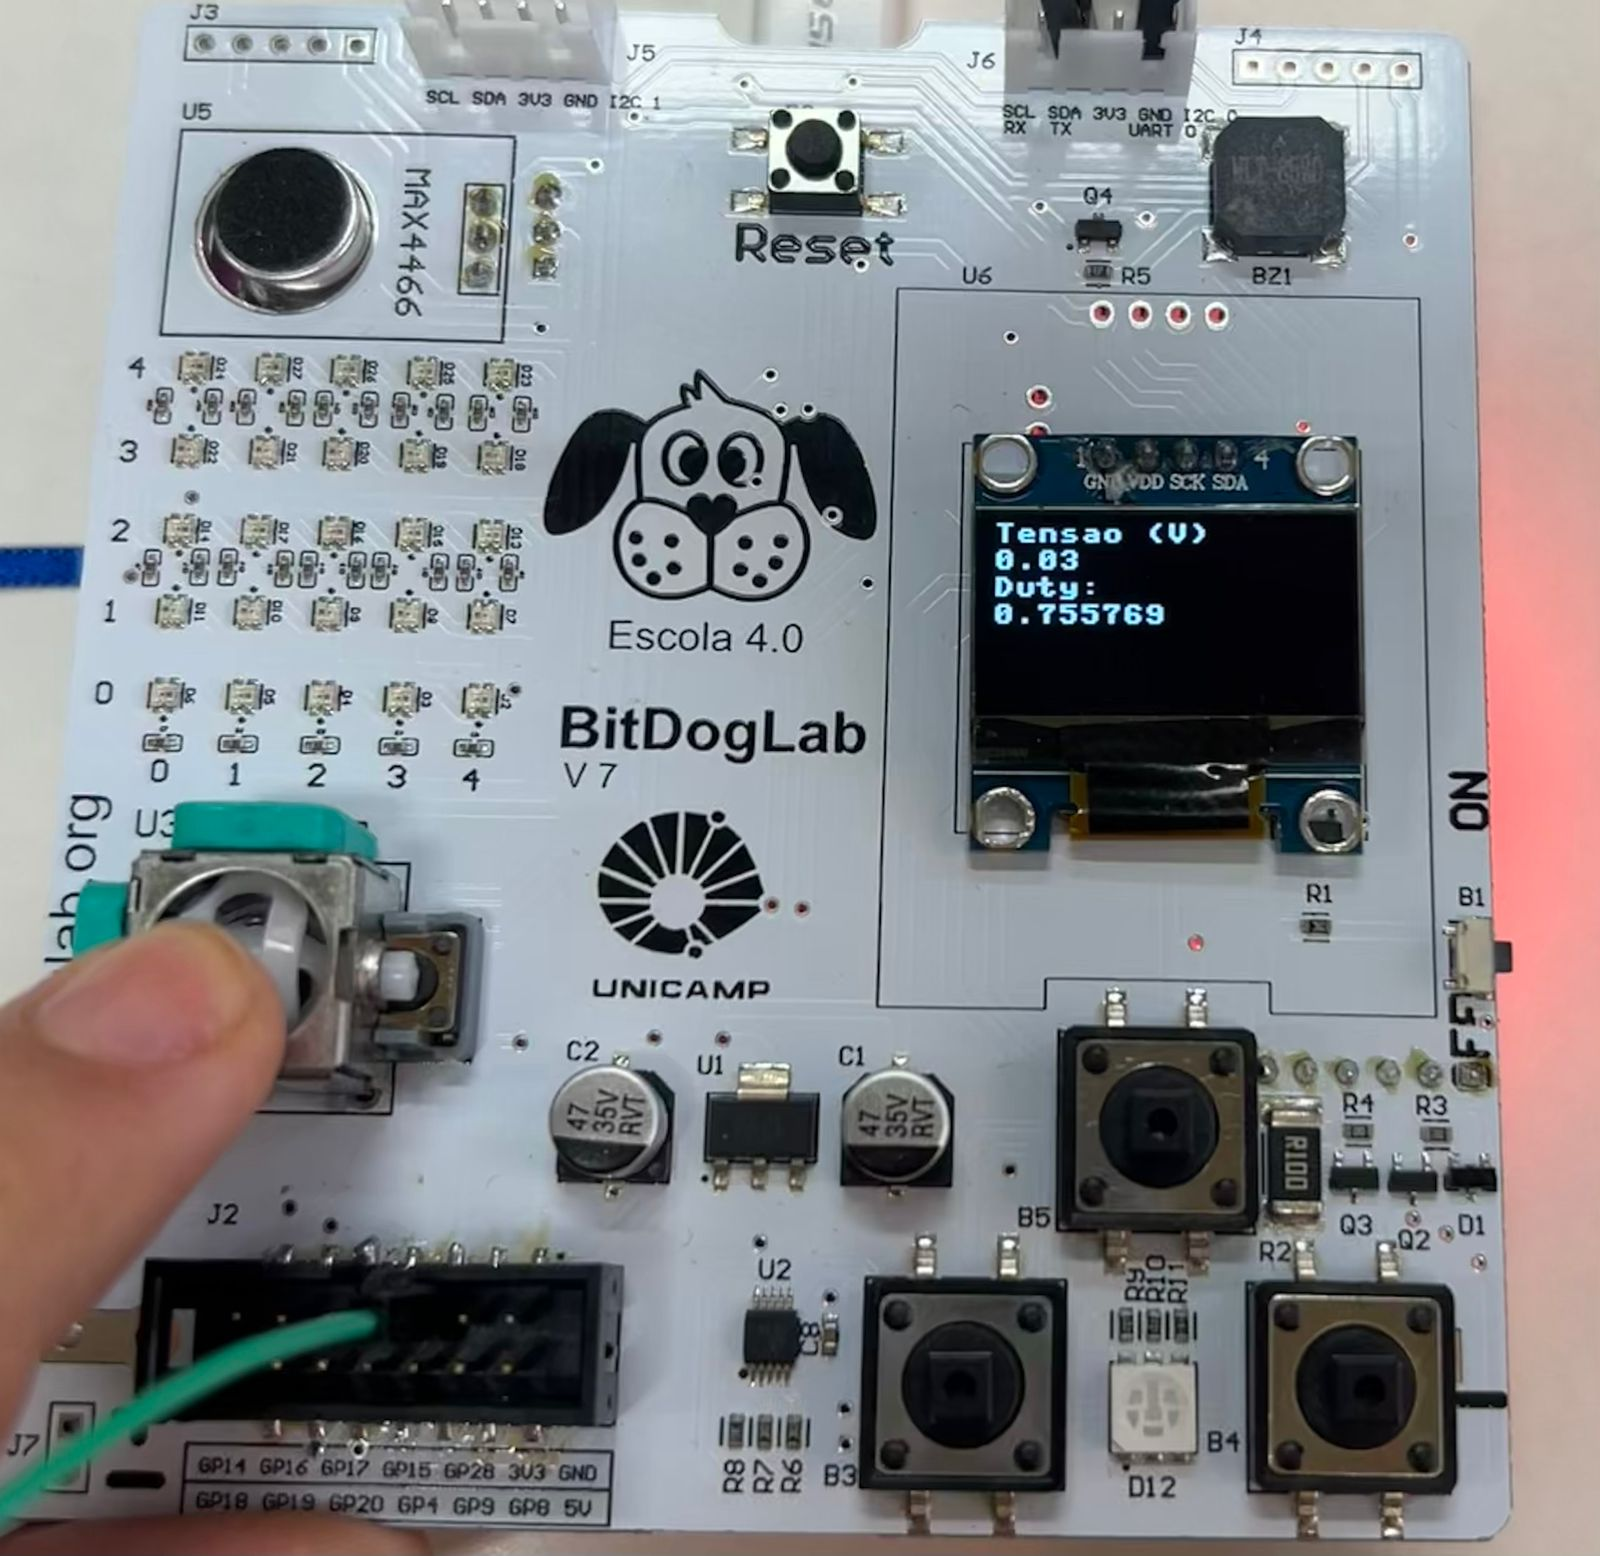
\includegraphics[width=\linewidth]{foto1.jpeg}
        \caption{Imagem no OLED com duty próximo a 0\%}
        \label{fig:foto1}
    \end{minipage}
    \hfill
    \begin{minipage}{0.45\linewidth}
        \centering
        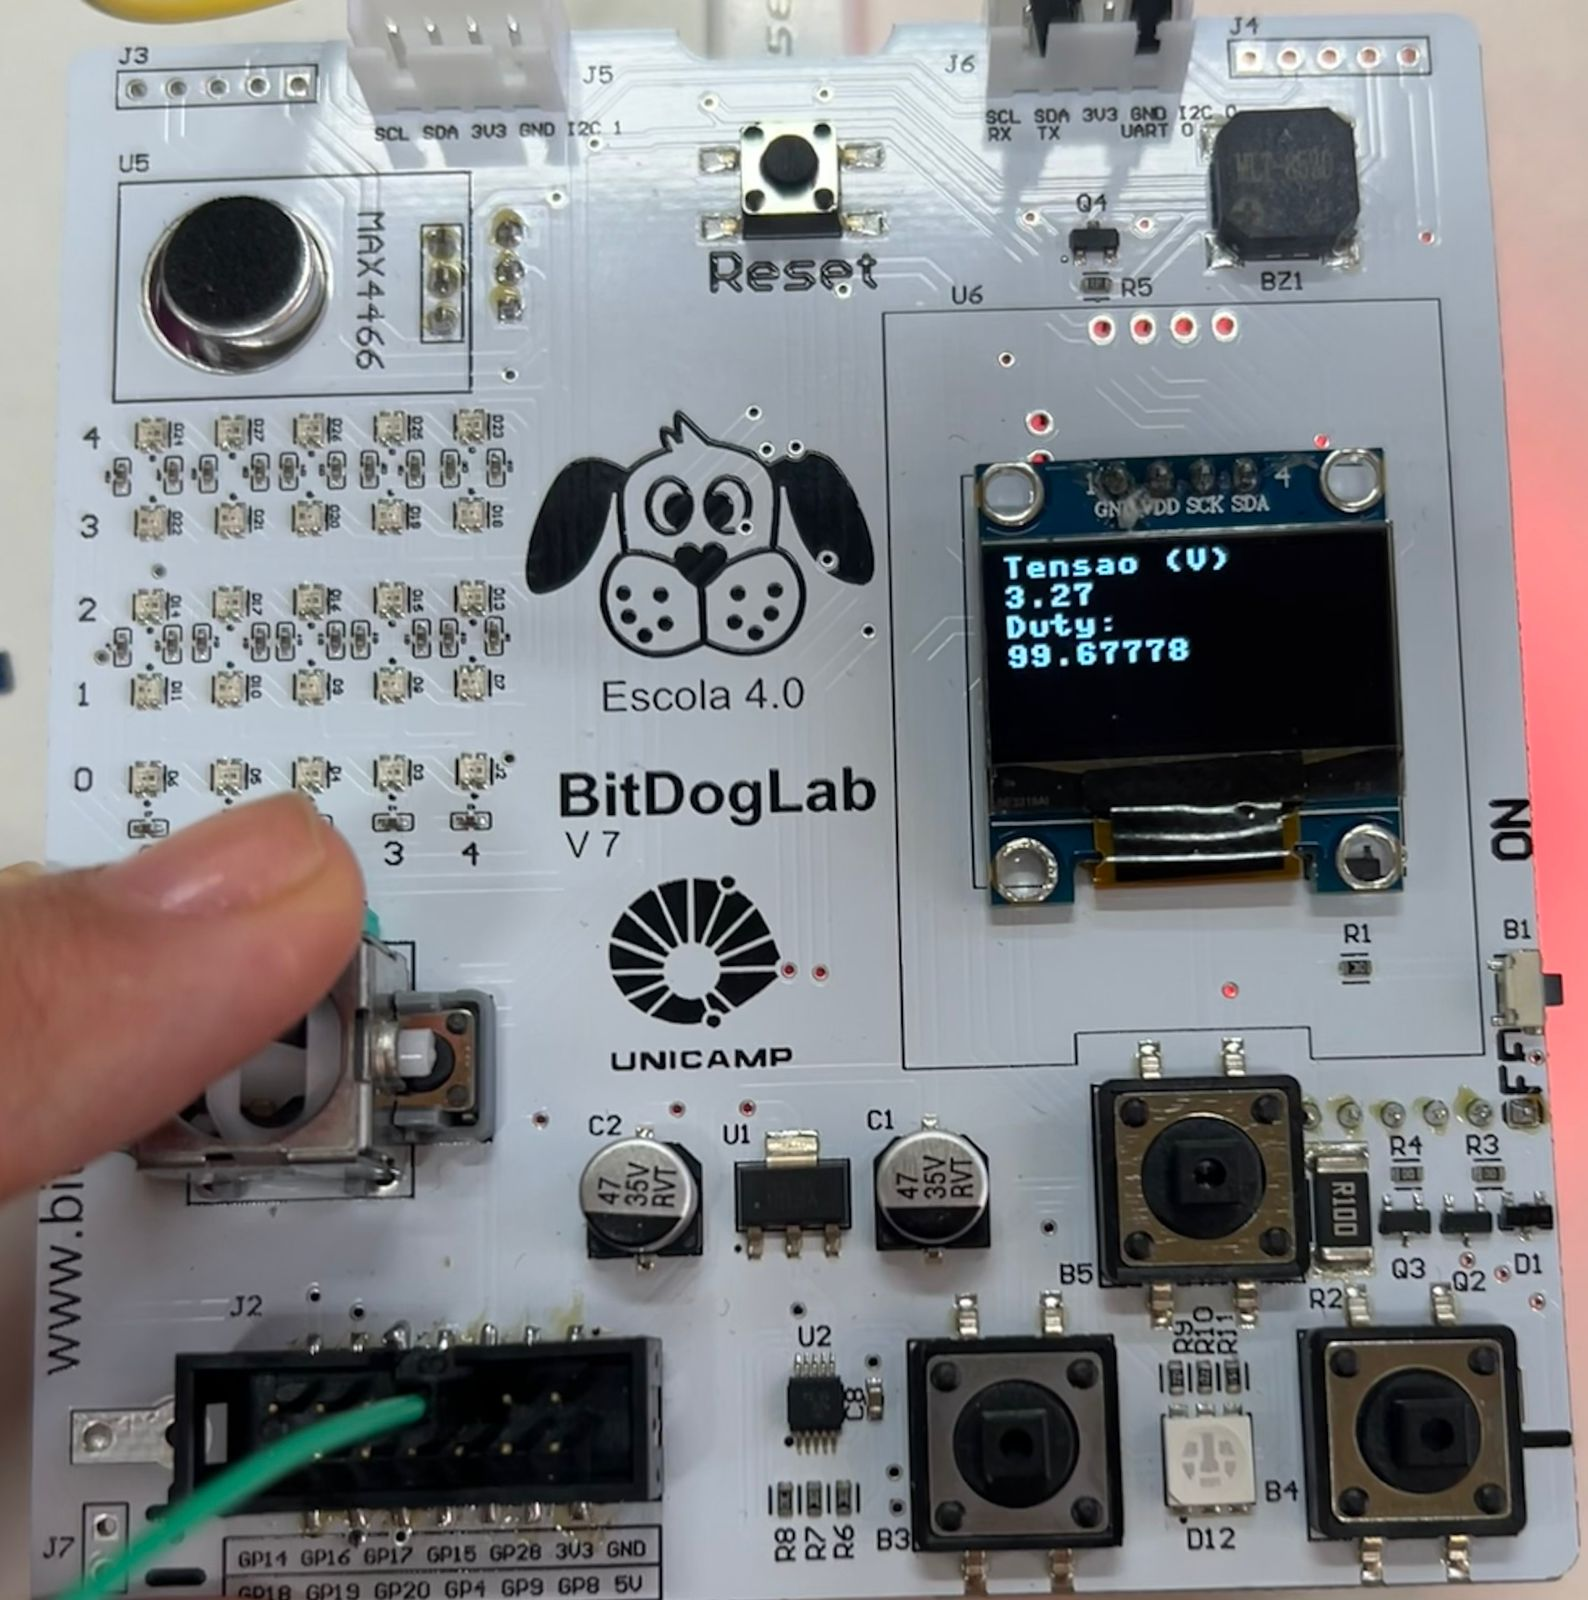
\includegraphics[width=\linewidth]{foto2.jpeg}
        \caption{Imagem no OLED com duty próximo a 100\%}
        \label{fig:foto2}
    \end{minipage}
\end{figure}

\subsection{PWM controlado pelo Joystick}

\begin{itemize}
    \item Usar \texttt{GPIO0} (ou \texttt{GPIO1}) como saída PWM.
    \item Controlar o duty cycle com o eixo X (0--100\%).
    \item Controlar a frequência com o eixo Y (100 Hz -- 20 kHz).
    \item Exibir no OLED: Duty (\%) e Frequência (Hz).
    \item Medir o sinal com o osciloscópio ou multímetro em modo de duty/frequência.
    \item \textbf{Observação:} reaproveite do experimento anterior.
\end{itemize}

\noindent
\textbf{Exercício:} variar o joystick e observar no display e no osciloscópio a mudança em tempo real. Observe que varia em toda a escala. 

\subsection{Filtro RC e Conversão Digital–Analógica}

\begin{itemize}
    \item Montar na protoboard um filtro RC passa-baixa:
    \begin{itemize}
        \item Exemplo: R = 10 k$\Omega$ e C = 100 nF $\rightarrow$ $f_c \approx 160$ Hz.
    \end{itemize}
    \item Conectar o PWM (\texttt{GPIO0}) à entrada do filtro.
    \item Saída do filtro $\rightarrow$ conectar ao ADC (\texttt{GPIO28}).
    \item Mostrar no OLED a tensão média medida pelo ADC e comparar com o valor esperado pelo duty cycle.
\end{itemize}

\section{Passo 1 - Configuração}

\begin{itemize}
    \item Monte um filtro RC passa-baixas. 
    \begin{itemize}
        \item Valores sugeridos: R = 10 k$\Omega$, C = 100 nF ($f_c \approx 160$ Hz).
    \end{itemize}
    \item Configure a entrada analógica: saída do filtro RC conectada ao ADC (\texttt{GPIO28}). 
    \begin{itemize}
        \item \textbf{Obs:} certifique-se em mudar a posição do jumper que conecta o \texttt{GPIO28} ao microfone, trazendo para os pontos de conexão externa (barra de terminal ou conector IDC).
    \end{itemize}
    \item Configure o \texttt{GPIO0} para gerar um sinal PWM variando o duty cycle de 0\% a 100\%, em passos de 10\%. Defina uma frequência adequada.
\end{itemize}

\section{Passo 2 - Tabela de medições}

\noindent
Crie uma planilha com uma tabela. Para cada duty:

\begin{itemize}
    \item Meça a tensão na saída do filtro (multímetro ou ADC $\rightarrow$ OLED).
    \item Calcule a tensão esperada: 
    \begin{equation}
        V_{exp} = V_{DD} \times \frac{Duty}{100}
    \end{equation}

    \item Plote o gráfico:
    \begin{itemize}
        \item Eixo $x$: duty cycle.
        \item Eixo $y$: tensão medida ($V_{exp}$).
    \end{itemize}
\end{itemize}

\begin{table}[ht!]
    \centering
    \begin{tabular}{|l|c|c|c|}
        \toprule
        Duty (\%) & Valor medido (V)& Valor esperado (V) & Erro ($V_{exp} - V_{obt}$) \\
        \midrule
        0 & 0 & 0 & 0 \\
        15 & 0.49 & 0.495 & 0.005 \\
        30 & 0.98 & 0.99 & 0.01 \\
        50 & 1.65 & 1.65 & 0 \\
        65 & 2.12 & 2.145 & 0.025 \\
        75 & 2.51 & 2.475 & 0.035 \\
        100 & 3.29 & 3.3 & 0.01  \\
         \bottomrule
    \end{tabular}
    \caption{Tabela com os valores medidos}
    \label{tab:medidas}
\end{table}

\begin{figure}[H]
    \centering
    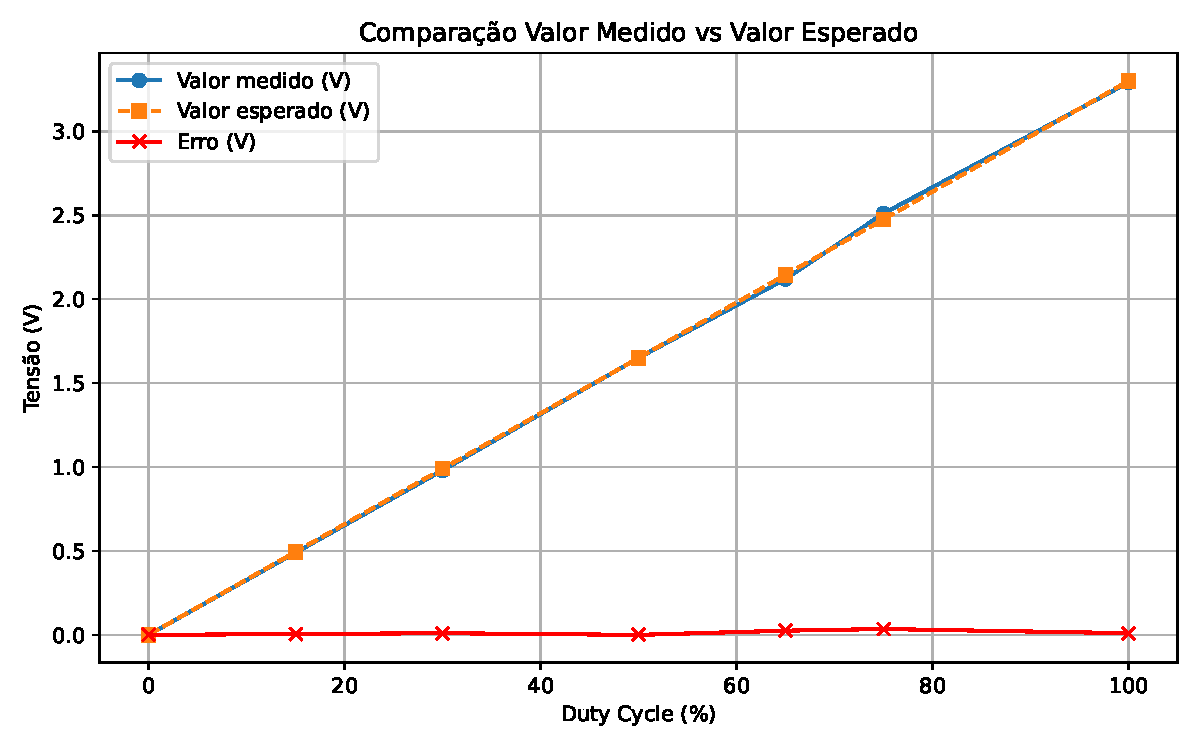
\includegraphics[width=0.8\linewidth]{grafico_duty.pdf}
    \caption{Gráfico comparando os valores obtidos e esperados}
    \label{fig:grafico}
\end{figure}

\noindent
\textbf{Resposta:} A Tabela \ref{tab:medidas} apresenta os valores medidos, os valores teóricos esperados e o respectivo erro. Observa-se que o erro obtido é relativamente baixo, considerando o método utilizado para a geração do sinal analógico. Já o Gráfico \ref{fig:grafico} evidencia a diferença entre os valores obtidos e os esperados, bem como o erro em cada ponto, mostrando que em todos os casos o erro permaneceu abaixo de 40 mV.

\section{Passo 3 - Gráfico de erro}

\noindent
Depois de preencher suas medições, crie um gráfico de erro  vs duty (\%). Use o eixo secundário y para mostrar o gráfico de erro.

\noindent
Com o valor medido para cada ponto, calcule: 

\begin{equation}
    \text{Erro (V)} = V_{med} - V_{exp}
\end{equation}
\begin{equation}
    \text{Erro (\%)} = 100 \times \frac{V_{med} - V_{exp}}{V_{DD}}
\end{equation}

\noindent
\textbf{Resposta:} A Figura \ref{fig:graficodeerro} apresenta o gráfico comparando o erro percentual em função do duty cycle (\%).

\begin{figure}[ht!]
    \centering
    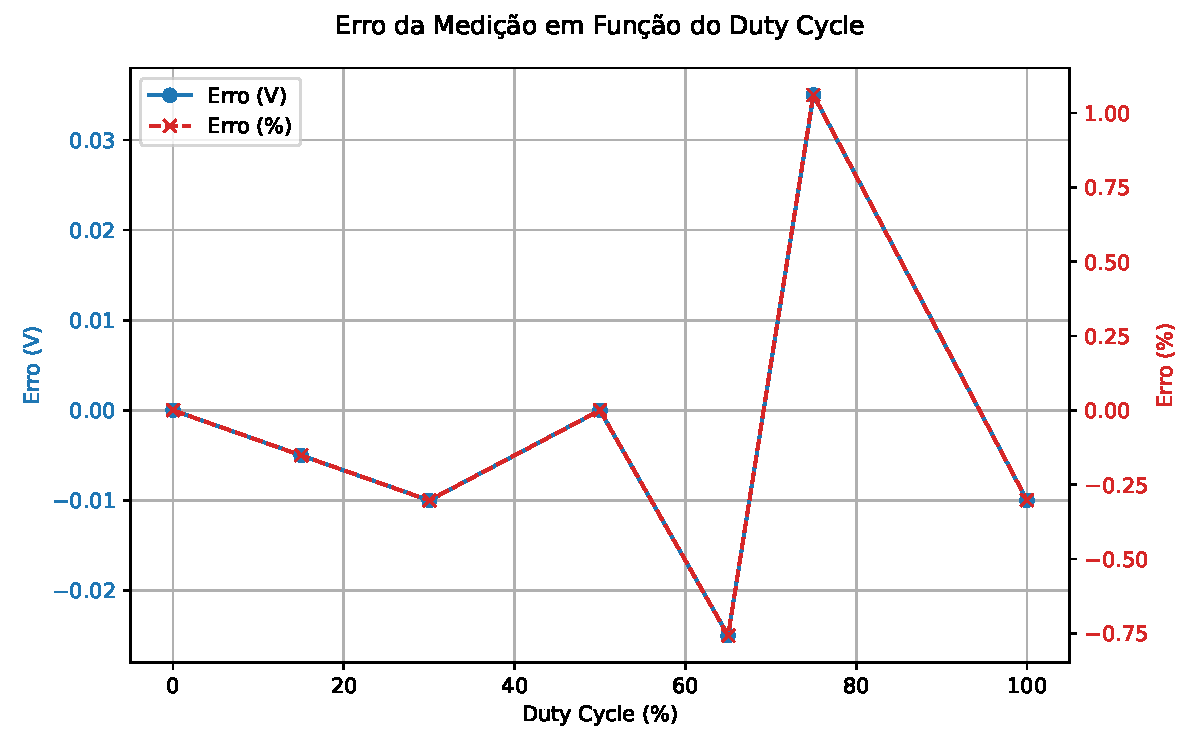
\includegraphics[width=0.9\linewidth]{erro_medição.pdf}
    \caption{Gráfico de erro}
    \label{fig:graficodeerro}
\end{figure}

\subsection{Dicas para boa qualidade das medições}

\begin{itemize}
    \item Aguarde alguns milissegundos após mudar o duty para o RC estabilizar ($\approx 3$--$5 \cdot RC$).
    \item Meça em múltiplos pontos e use a média para reduzir ruído.
    \item Para reduzir ripple:
    \begin{itemize}
        \item Aumente a frequência do PWM, ou
        \item Aumente $C$ (com cuidado, a resposta ficará mais lenta).
    \end{itemize}
    \item Documente a frequência do PWM utilizada — faz diferença no ripple.
\end{itemize}

\noindent
\textbf{Resposta:} Utilizou-se uma frequência de 10 kHz; anteriormente, havia sido utilizada uma frequência de 1 kHz. É perceptível uma redução considerável no efeito de ripple ao aumentar a frequência. As figuras \ref{fig:lowduty}, \ref{fig:halfduty} e \ref{fig:fullduty} ilustram a saída observada no osciloscópio para diferentes valores de duty cycle — respectivamente 0\%, 50\% e 100\% — mostrando que o ripple atingiu valores mínimos em todas as condições.

\begin{figure}
    \centering
    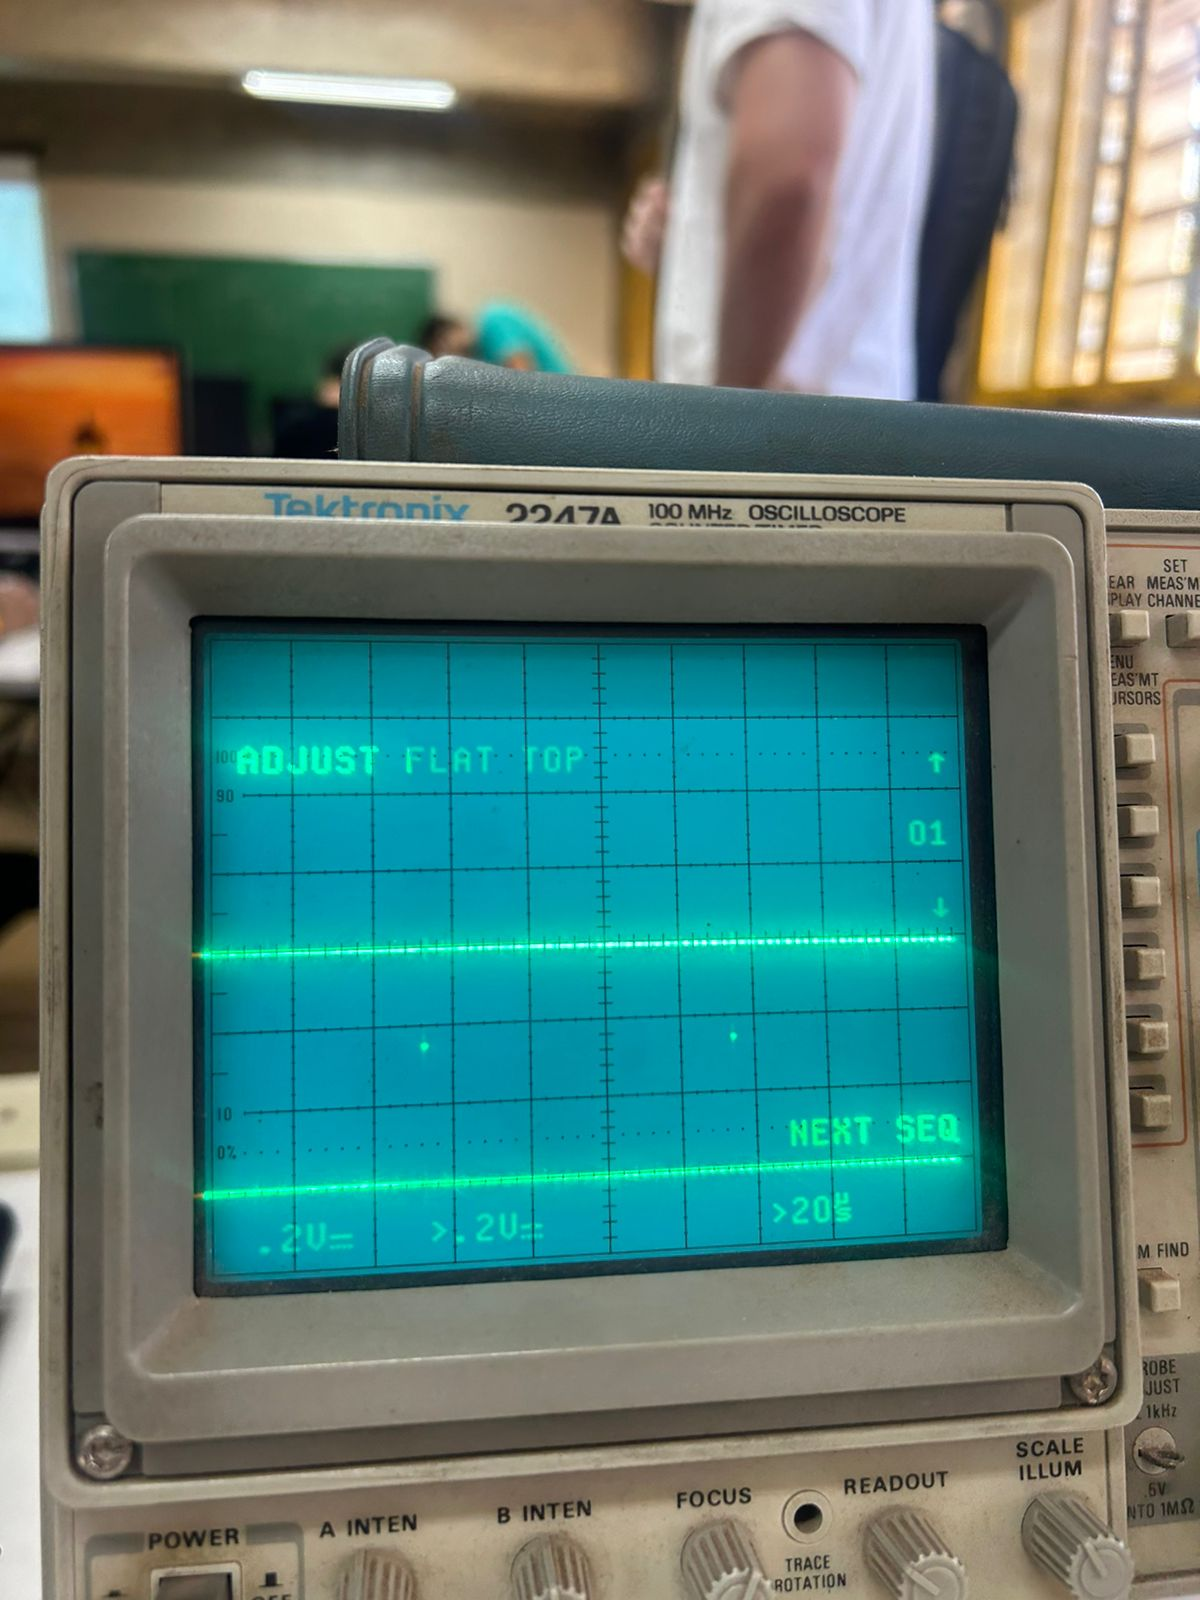
\includegraphics[width=0.9\linewidth]{low_duty.jpeg}
    \caption{Duty em 0\%}
    \label{fig:lowduty}
\end{figure}

\begin{figure}
    \centering
    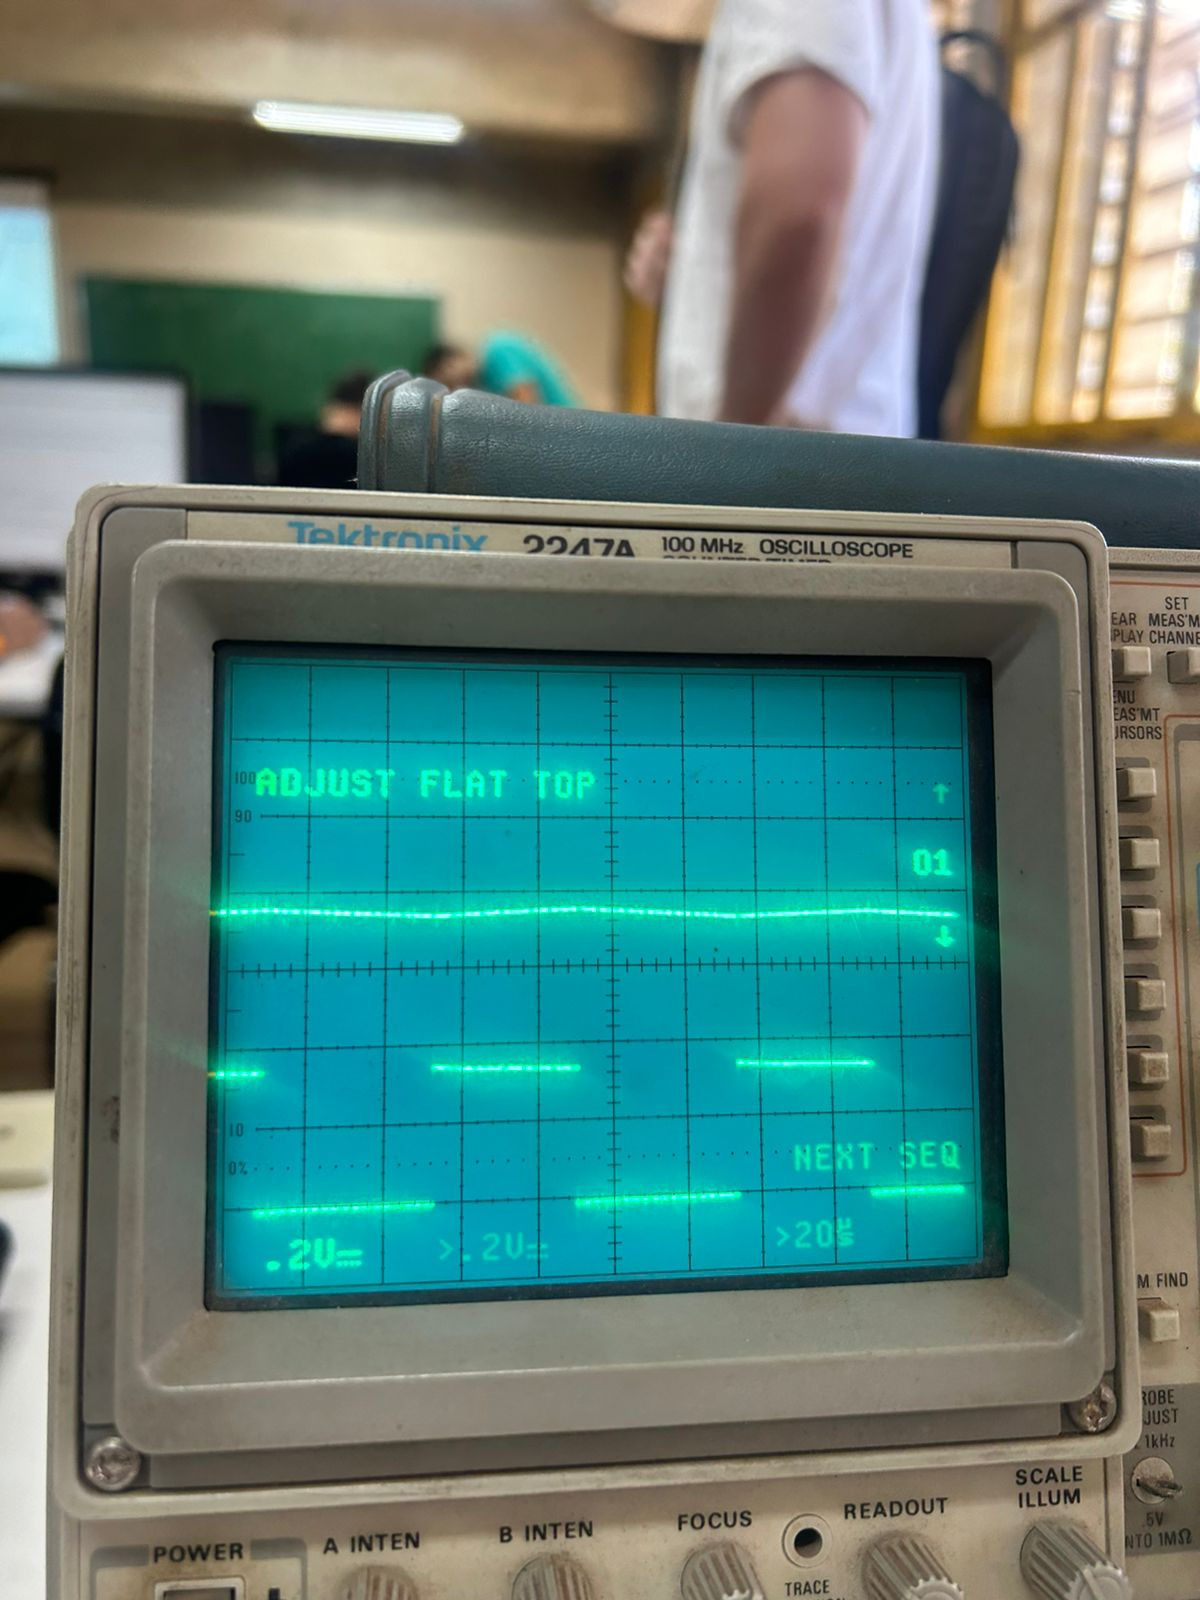
\includegraphics[width=0.9\linewidth]{half_duty.jpeg}
    \caption{Duty em 50\%}
    \label{fig:halfduty}
\end{figure}

\begin{figure}
    \centering
    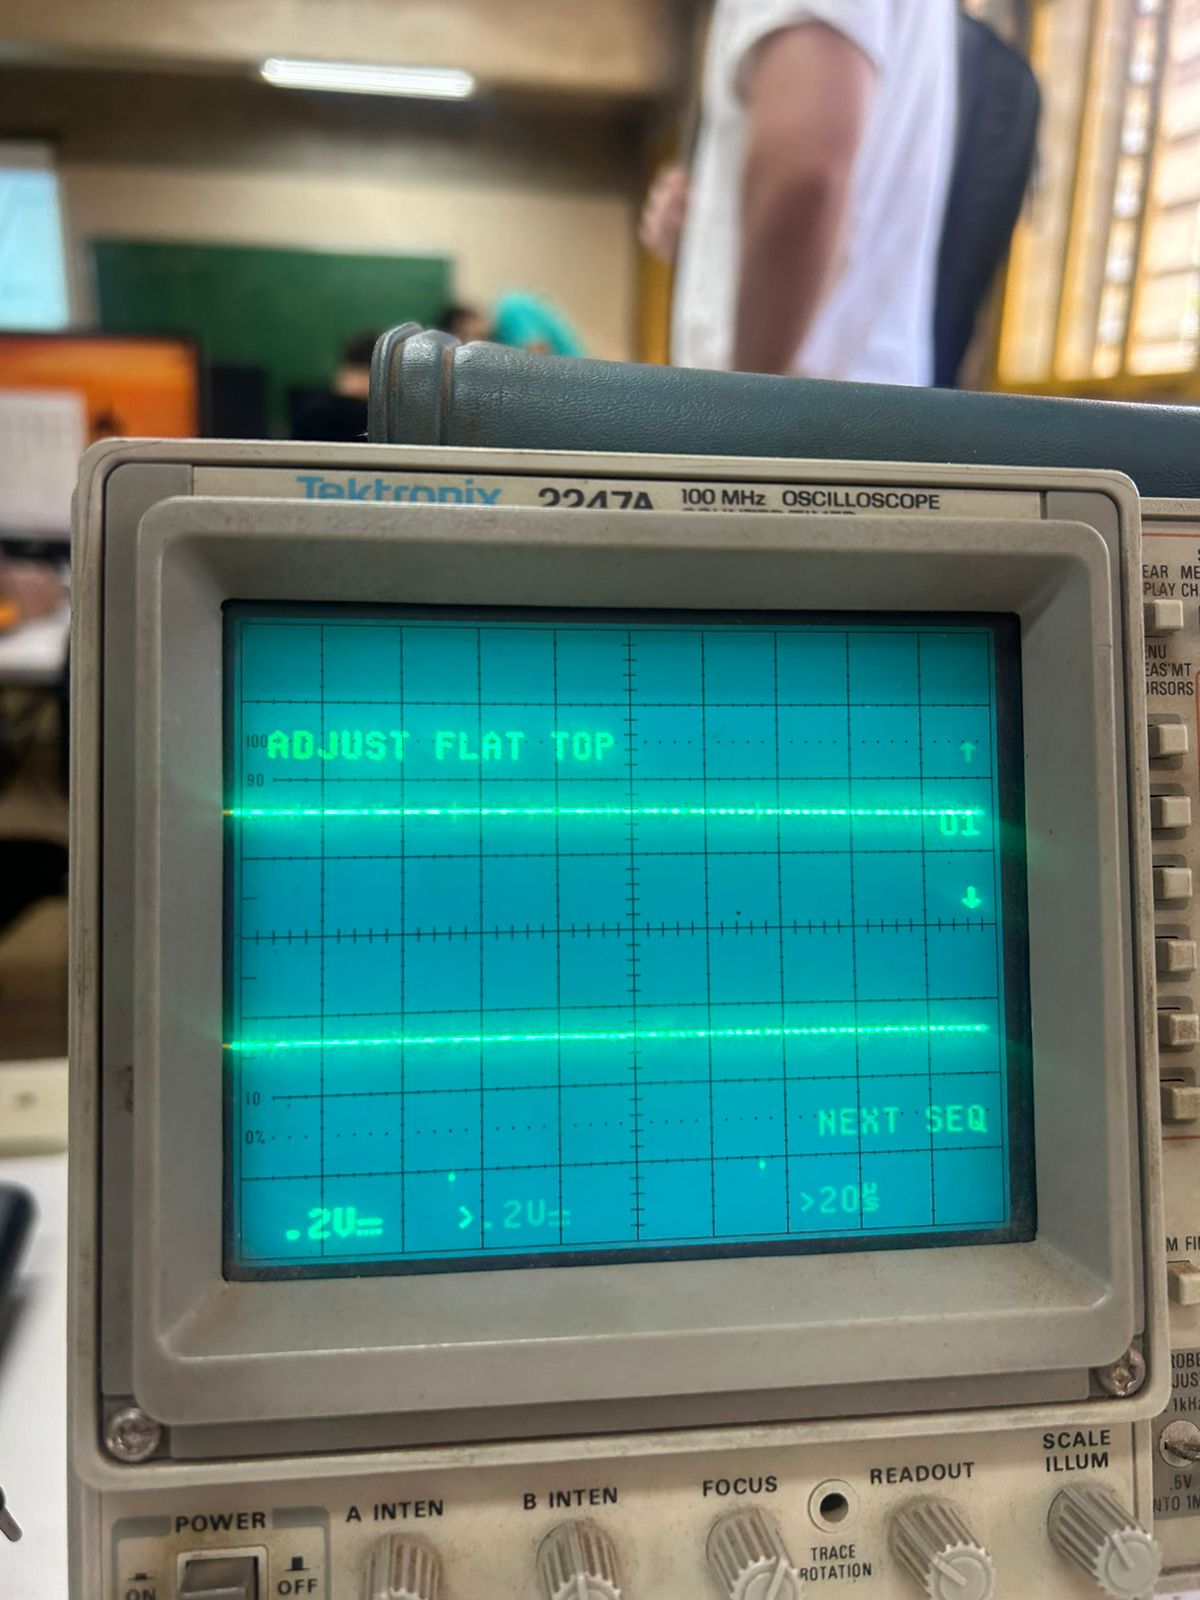
\includegraphics[width=0.9\linewidth]{full_duty.jpeg}
    \caption{Duty em 100\%}
    \label{fig:fullduty}
\end{figure}

\end{document}
